\documentclass[../../dissertation.tex]{subfiles}
\begin{document}

\subsection{Grover}
As was previously seen in section \ref{sec:GrovSearchSimul}, Grover's algorithm
is a quantum alternative to unstructured search problems. Consider the case of
finding element $x_0$ out of an unordered list of size $N$. Worst case
scenario, a classical algorithm would need to check every element of the list,
requiring $N$ steps.\par

The first stage of Grover's algorithm is to create an uniform superposition of
all states in the system
\begin{equation}
	\ket{\Psi_0}  = \frac{1}{\sqrt{N}}\sum_{x=0}^{N-1} \ket{x}.
\end{equation}\par
The next stage is the application of the Grover iteration process, which starts
with an oracle that adds a negative phase to the solution states
\begin{equation}
        \mathcal{O}\ket{x} = (-1)^{f(x)}\ket{x}.
\end{equation}
This operator can be seen as an identity matrix with negative entries
corresponding to the solution states, and the operator can be rewritten as 
\begin{equation}
	\mathcal{O} = I - 2\sum_{m\in M} \ket{m}\bra{m}.
	\label{eq:groverQiskitOracle}
\end{equation}
where $I$ is the identity matrix and $M$ is a set of solutions where $f(m) =
1$, otherwise it's $0$. The matrix associated with this operator will be
\begin{equation}
	\mathcal{O} = 
	\begin{pmatrix}
		(-1)^{f(0)} & 0 & \cdots & 0\\
	        0 & (-1)^{f(1)} & \cdots & 0\\ 
	        \vdots & 0 &  \ddots & \vdots\\ 
		0 & 0 & \cdots &  (-1)^{f(N-1)}
	\end{pmatrix}.
	\label{eq:oracleMatrixQiskit}
\end{equation}\par
%TODO: Mencionar que o grover se extende a toda a categoria de problemas que envolvam aquela matriz.
The second part of the iteration is an amplitude amplification process by means
of the diffusion operator 
\begin{equation}
        %TODO: Decidir se mantenho os H's.
        \mathcal{D} = (2\ket{\Psi_0}\bra{\Psi_0} - I) = H^{\otimes n}(2\ket{0}\bra{0} - I)H^{\otimes n}.
	\label{eq:groverQiskitDiffusion}
\end{equation}
The unitary operator that describes the Grover iteration process will then be
\begin{equation}
        \mathcal{U} = \mathcal{D}\mathcal{O}.
\end{equation}\par

As was previously discussed, this iteration process will be done several times,
depending on the number of elements. Optimal probability of success finding a
single solution will be reached after $\floor{\frac{\pi}{4}\sqrt{N}}$ steps,
and $\floor{\frac{\pi}{4}\sqrt{\frac{N}{K}}}$ for $K$ solutions, which is a
quadratic gain when compared to the classical case. The general Grover circuit
can then be constructed as is shown in figure \ref{fig:groverSearchCircuit}.
\begin{figure}[!h]
	\[ \Qcircuit @C=1.8em @R=1.5em {& & & && \mbox{ Repeat $O(\sqrt{N})$ times}  & & &\\
	& & {/^{\otimes n}} \qw &\gate{H}  & \gate{\mathcal{O}} &  \gate{D} & \qw &\qw \gategroup{2}{5}{2}{6}{.8em}{--}
		          } \]
	\centering
	\caption{General circuit for the Grover search.}
	\label{fig:groverSearchCircuit}
\end{figure}\par
Consider the $3$ qubit case, where $N=8$ and solution state $\ket{4}$. The
optimal number of iterations is approximately $2$, and figure
\ref{fig:groverCircuitQistkit} is the circuit for $3$ iterations implemented in
Qiskit.
\begin{figure}[!h]
	\centering
	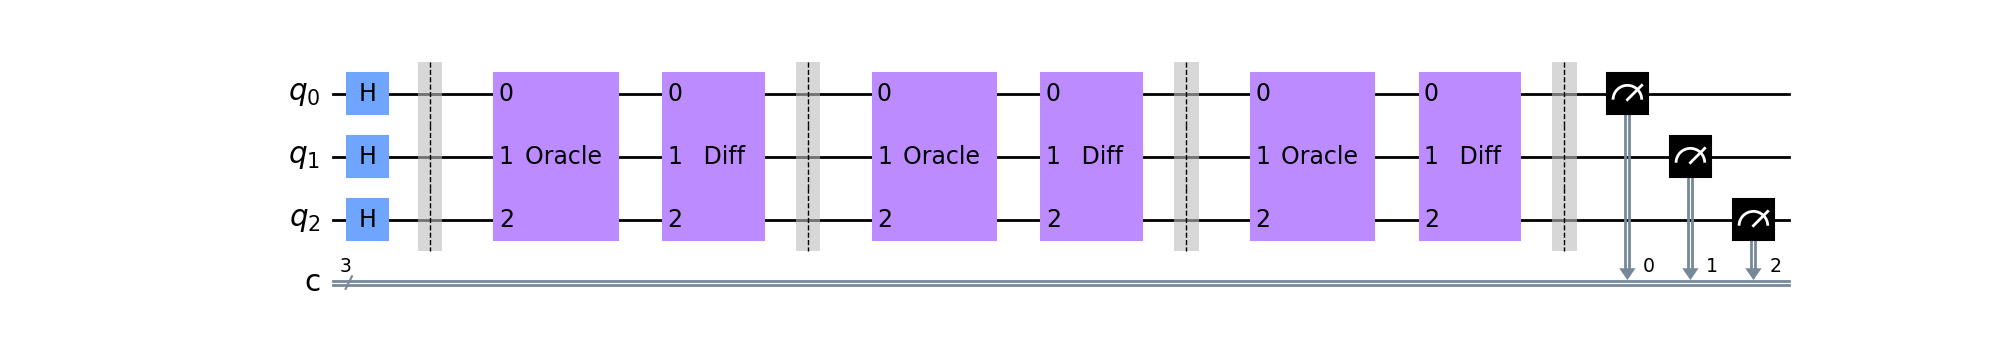
\includegraphics[scale=0.32]{img/Qiskit/GroverQiskit/Circuits/GroverQiskitCirc_N3_M4_S3.png}
	\caption{Qiskit circuit for the Grover algorithm, for a search size of $N=8$ and $3$ steps.}
	\label{fig:groverCircuitQistkit}
\end{figure}\par
%TODO:Melhorar 
The system starts with the creation of an uniform superposition state, which
means applying Hadamard gates to each qubit.  
\begin{figure}[!h]
	\centering
	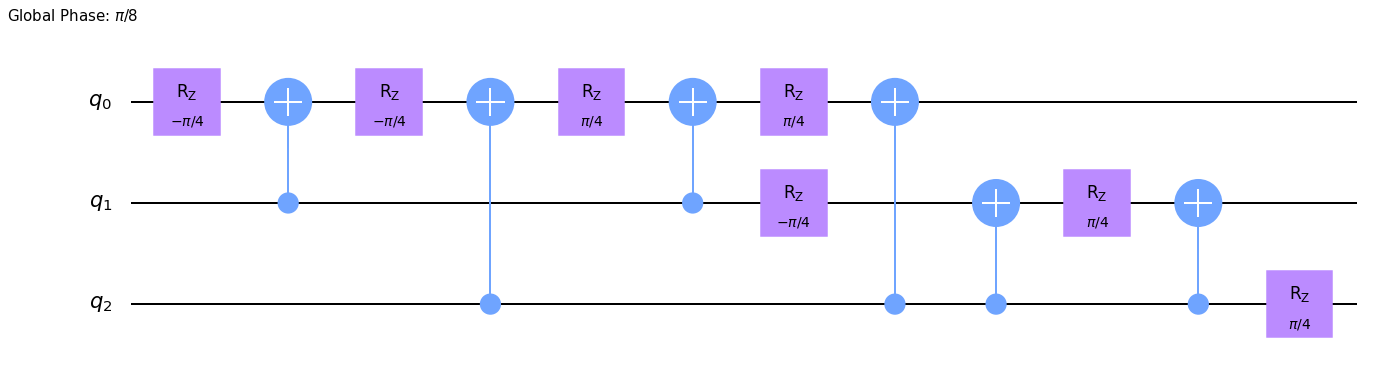
\includegraphics[scale=0.25]{img/Qiskit/GroverQiskit/Circuits/GroverQiskitCircOracle_N3_M4_S3.png}
	\caption{Qiskit circuit of the  diagonal oracle operator in search space of size $N=8$, for marked element $\ket{m}=\ket{4}$.}
	\label{fig:groverOracleCircuitQistkit}
\end{figure}
Immediately following the barrier, the first operator of the iteration process
is the oracle, which is shown in figure \ref{fig:groverOracleCircuitQistkit}.
Because the oracle operator is simply the identity matrix with negative entries
corresponding to the solution states, it can be simply translated into a
circuit by means of the \textit{diagonal} function in Qiskit.\par

The last part of the iteration is the diffusion operator, whose circuit is
shown in figure \ref{fig:groverDiffCircuitQistkit}.
\begin{figure}[!h]
	\centering
	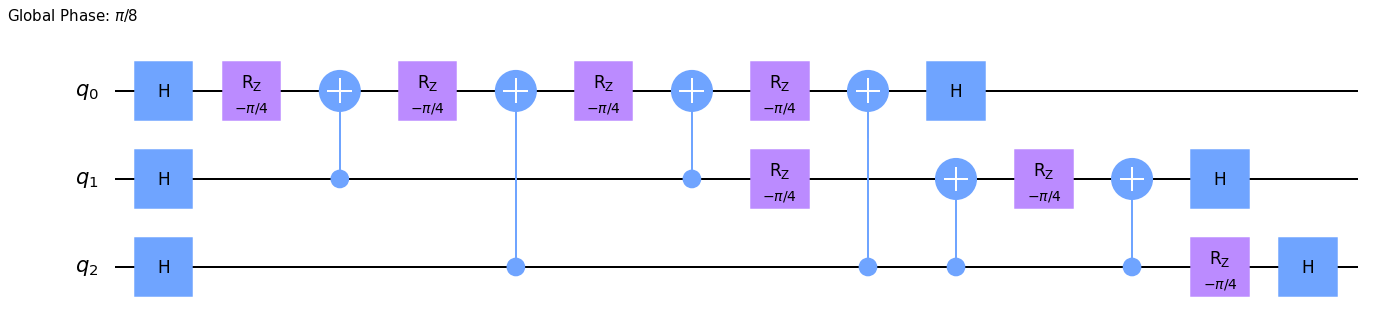
\includegraphics[scale=0.25]{img/Qiskit/GroverQiskit/Circuits/GroverQiskitCircDiff_N3_M4_S3.png}
	\caption{Qiskit circuit of the  diagonal Grover diffusion operator in search space of size $N=8$.}
	\label{fig:groverDiffCircuitQistkit}
\end{figure}
%TODO Isto esta muito fraco. 
Comparing equations \ref{eq:groverQiskitOracle} and
\ref{eq:groverQiskitDiffusion}, it is easy to see why figures
\ref{fig:groverOracleCircuitQistkit} and \ref{fig:groverDiffCircuitQistkit} are
so similar. The diffusion circuit will simply be the oracle circuit for state
$\ket{0}$ in between Hadamard operations.
\begin{figure}[!h]
	\centering
	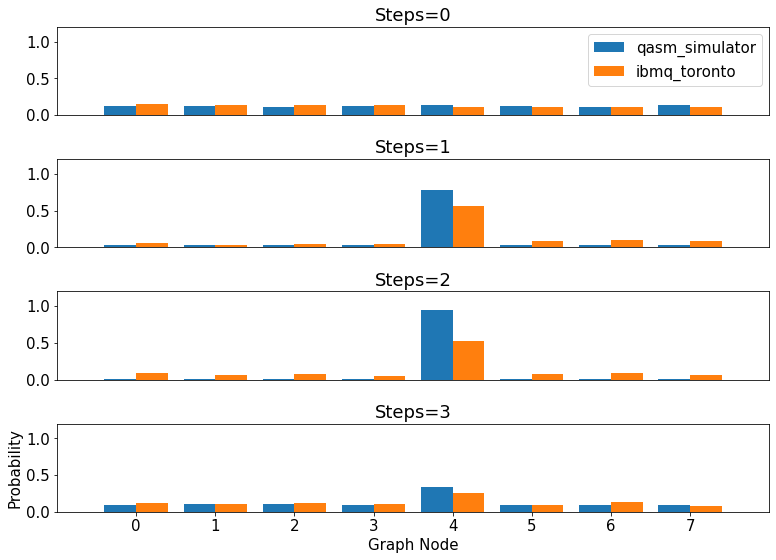
\includegraphics[scale=0.40]{img/Qiskit/GroverQiskit/GroverQiskitSearch_N3_M4_S0123}
	\caption{Probability distributions of the Grover search algorithm for several steps, in a search space of size $N=8$. The blue bar plot represents a circuit run in the QASM simulator, and the orange bar plot on IBM's Toronto backend.}
	\label{fig:groverQiskitDist}
\end{figure}\par

The results of measurement are shown in figure \ref{fig:groverQiskitDist}. As
was expected, maximum probability for the marked element was reached after $2$
iterations, on the simulator, and it decreases in subsequent steps. However,
the experimental result from the Toronto backend present maximum probability
for the marked element for $1$ step, with a fidelity of $0.96$. The optimal
number of steps, in contrast, have a lower fidelity of $0.89$. This is because
as the number of steps increases, so does circuit depth, meaning that the
circuit does not achieve the maximum probability after $2$ steps due to the
effects introduced by noise.\par

Despite the effects introduced by noise, the results are satisfactory when
considering the properties of NISQ computers. The following sections will
present the search problem adapted to several quantum walk models.

\subsection{Coined}
Following the structure of section \ref{sec:CoinedSearchSimul}, this chapter
aims to expand the coined quantum walk model by incorporating concepts like the
oracle and diffusion operator of the Grover search, with the purpose of generating a quantum circuit that performs this algorithm.\par 

The modified unitary evolution operator is
\begin{equation}
        U' = S (\mathcal{O} \otimes G),\label{eq:modifiedEvoCoinedQiskit}
\end{equation}
%TODO: Relembrar equacoes para cada um dos operadores? Parece me desnecessario.
as was defined in equation \ref{eq:modifiedEvoCoined}, where $S$ is the
flip-flop shift operator, $\mathcal{O}$ is the oracle operator and $G$ is the
Grover diffusion as a coin operator.\par

Consider the case of a complete graph, where every vertex is adjacent to one
another. The general quantum circuit to implement this, as shown in figure
\ref{fig:coinedSearchCircuit}, will require $n$ qubits to represent the state
of the walker and $n$ qubits for the state of the coin.  The shift operator was
constructed based on the work of \cite{douglaswang07}, where the state of the
walker is flip-flopped with the state of the coin by means of the swap
operation.
\begin{figure}[!h]
	\[ \Qcircuit @C=1.8em @R=1.5em { & & & & \mbox{ Repeat $O(\sqrt{N})$ times}  &\\
	                                & {/^{\otimes n}} \qw  &\gate{H}  & \gate{\mathcal{O}} & \multigate{1}{SHIFT} & \qw &  \\
				                    & {/^{\otimes n}} \qw  & \qw & \gate{G}&   \ghost{SHIFT} & \qw \gategroup{2}{4}{3}{5}{.8em}{--}
		          } \]
	\centering
	\caption{General circuit for the search problem using the coined quantum walk model.}
	\label{fig:coinedSearchCircuit}
\end{figure}\par

This was implemented in Qiskit, for a graph of size $N=2^3=8$, which means $6$
qubits will be required. For the case of one marked element, the number of
iterations that maximizes the amplitude of the solution state is
$\floor{\frac{\pi}{2} \sqrt{N}}$, and figure
\ref{fig:coinedQWSearchCircuitQistkit} shows the circuit for 5 iterations of
the walk.
\begin{figure}[!h]
	\centering
	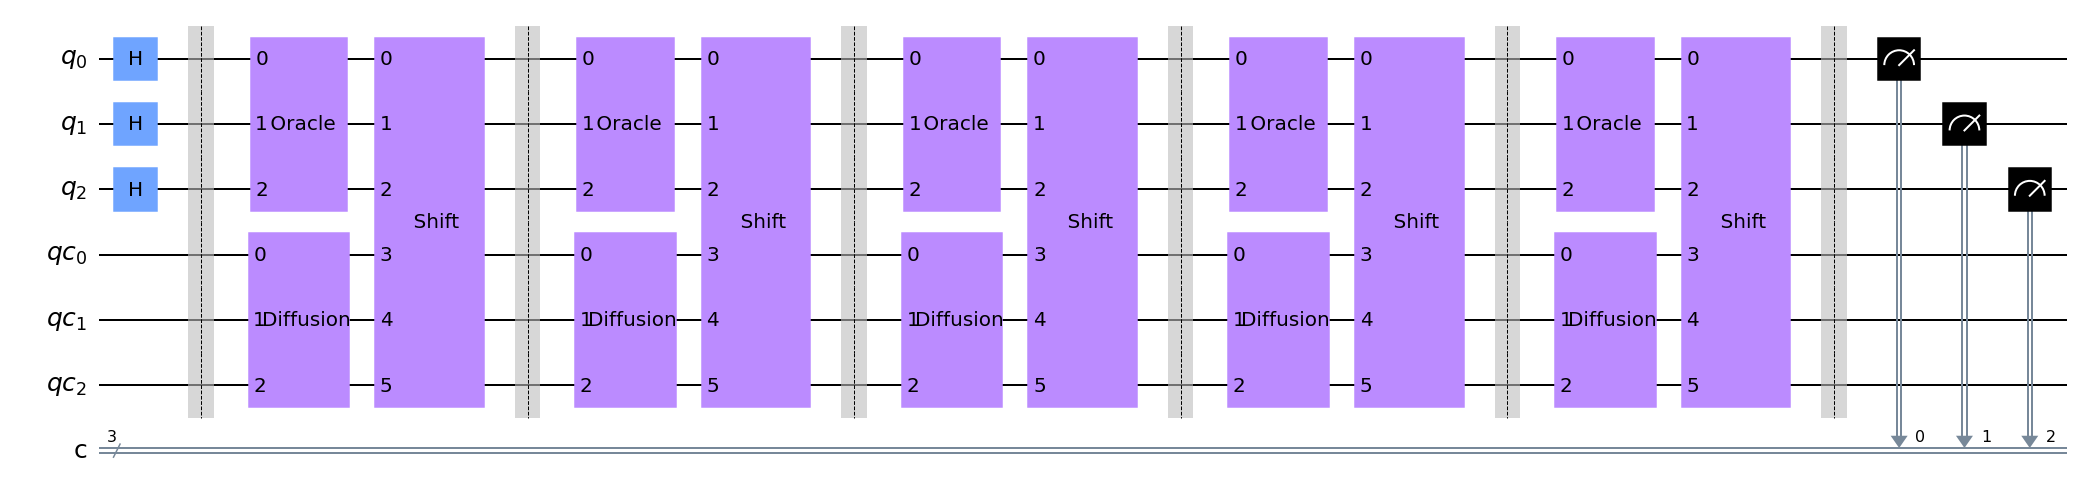
\includegraphics[scale=0.21]{img/Qiskit/CoinedQuantumWalk/Search/Circuits/CoinedSearchQiskitCirc_N3_M0_S5.png}
	\caption{Qiskit circuit for the search problem using the coined quantum walk model, for a complete graph of size $N=8$ and with $5$ steps.} 
	\label{fig:coinedQWSearchCircuitQistkit}
\end{figure}\par

The circuit starts in a uniform superposition of the states corresponding to
the vertices of the graph, and the first step of the iteration is the oracle.
This operator will flip the amplitude of the vertex state $\ket{4}$, and can be
translated to a circuit making use of Qiskit's \textit{diagonal}, as is shown
in figure \ref{fig:coinedQWSearchOracleCircuitQistkit}. 
\begin{figure}[!h]
	\centering
	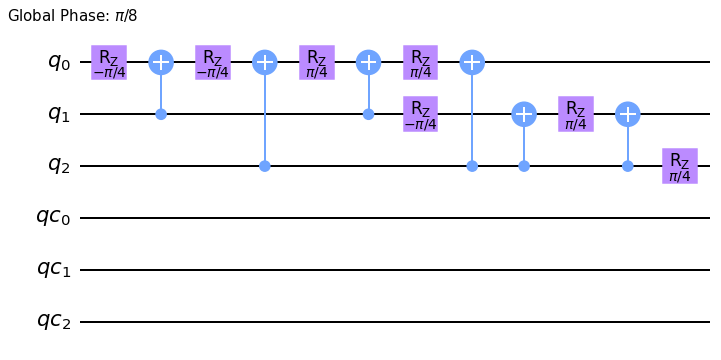
\includegraphics[scale=0.30]{img/Qiskit/CoinedQuantumWalk/Search/Circuits/CoinedSearchQiskitCircOracle_N3_M4_S5.png}
	\caption{Qiskit circuit of the  diagonal oracle operator in the coined quantum walk search problem, for a complete graph of size $N=8$, with marked element $\ket{m}=\ket{4}$.} 
	\label{fig:coinedQWSearchOracleCircuitQistkit}
\end{figure}
It is the same oracle as in the Grover search of figure
\ref{fig:groverOracleCircuitQistkit}, but in the coined quantum walk model it
is only applied to the states associated with the position of the walker. The
states associated with the coin space of the walk will be transformed according
to Grover's diffusion of figure \ref{fig:groverDiffCircuitQistkit}, as is seen
in figure \ref{fig:coinedQWSearchDiffCircuitQistkit}. 
\begin{figure}[!h]
	\centering
	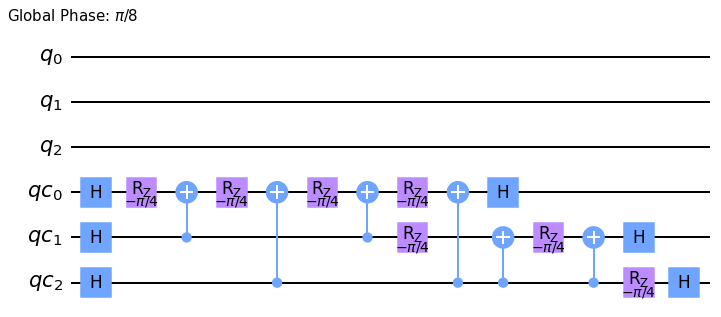
\includegraphics[scale=0.30]{img/Qiskit/CoinedQuantumWalk/Search/Circuits/CoinedSearchQiskitCircDiff_N3_M4_S5.png}
	\caption{Qiskit circuit of the  diagonal diffusion operator in the coined quantum walk search problem, for a complete graph of size $N=8$.} 
	\label{fig:coinedQWSearchDiffCircuitQistkit}
\end{figure}\par

The final part of the iteration is the shift operator, as can be seen in figure
\ref{fig:coinedQWSearchShiftCircuitQistkit}. The flip-flop shift operator was
defined in equation \ref{eq:chap3FlipFlop} as
\begin{equation}
        S\ket{v1}\ket{v2} = \ket{v2}\ket{v1},
        \label{eq:chap4FlipFlop}
\end{equation}
where $\ket{v1}$ represents the position of the walker and $\ket{v2}$ is the
state of the coin. Making use of the swap gate, this operator can be
implemented as in figure \ref{fig:coinedQWSearchShiftCircuitQistkit}.
\begin{figure}[!h]
	\centering
	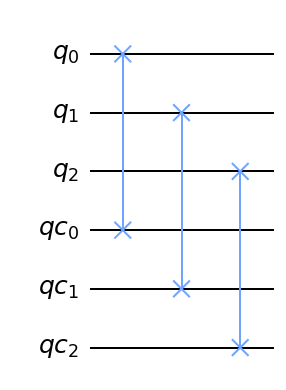
\includegraphics[scale=0.27]{img/Qiskit/CoinedQuantumWalk/Search/Circuits/CoinedSearchQiskitCircShift_N3_M4_S5.png}
	\caption{Qiskit circuit of the  flip-flop shift operator in the coined quantum walk search problem, for a complete graph of $N=8$.} 
	\label{fig:coinedQWSearchShiftCircuitQistkit}
\end{figure}\par
%TODO: Estudar porque e que a dist muda logo para 0 (diffusion) em steps = 5
%TODO: Melhorar texto.
Lastly, measurements were performed, and the results plotted in figure
\ref{fig:coinedSearchQiskitDist}. Maximum probability of the marked element was
reached after $4$ steps in the simulator, and extra steps reduce said
probability.  The resulting probability distribution from the Toronto backend
is again unsatisfactory for the coined quantum walk model, with fidelities
ranging from $0.58$ for $4$ steps, to $0.75$ for $2$ steps. This is expected,
since the complete graph representation requires $N$ extra qubits for the coin,
and swap operations which are decomposed into $3$ CNOTs each. The optimal
number of steps that maximizes the probability of the marked element is also a
contributing factor to the size of the circuit, requiring more iterations to
achieve the same probability when compared to Grover's search in the previous
chapter. 
\begin{figure}[!h]
	\centering
	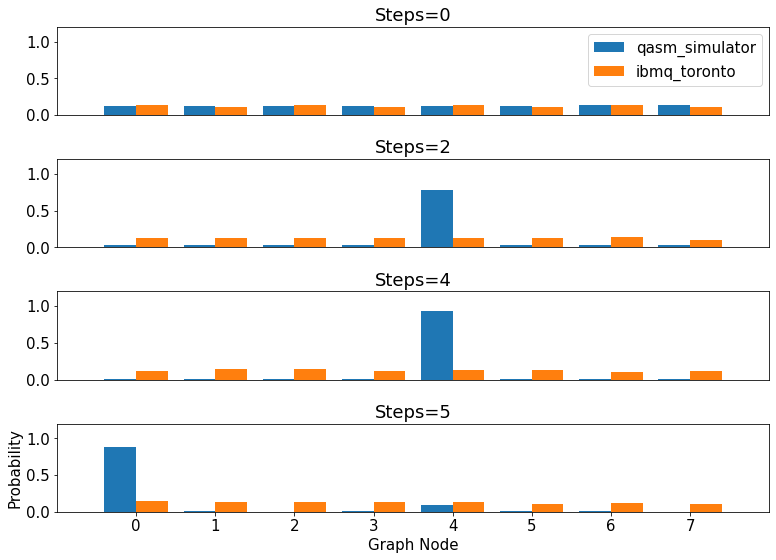
\includegraphics[scale=0.40]{img/Qiskit/CoinedQuantumWalk/Search/CoinedQiskitSearch_N3_M4_S0245}
	\caption{Probability distributions of the coined quantum walk search problem for several steps, in a complete graph of size $N=8$. The blue bar plot represents a circuit run in the QASM simulator, and the orange bar plot on IBM's Toronto backend.} 
	\label{fig:coinedSearchQiskitDist}
\end{figure}\par

As was done previously, other models of the quantum walks that do
not require coins or iterations will be studied in the following sections, in
the context of the searching problem. The staggered quantum walk, for example,
should be able to present better results when ran in a NISQ computer, considering the
smaller Hilbert space due to its coinless nature.

\subsection{Staggered}
Recalling from section \ref{sec:StagSearchSimul}, the staggered quantum walk on
a complete graph requires a single tessellation with associated polygon
\begin{equation}
	\ket{\alpha} = \frac{1}{\sqrt{N}} \sum_{x=0}^{N-1} \ket{x}.
\end{equation}
The Hamiltonian will then be 
\begin{equation}
	H_\alpha = 2\sum_0^1\ket{\alpha}\bra{\alpha} - I = H^{\otimes n} (2\ket{0}\bra{0} - I) H^{\otimes n} = H^{\otimes n} \mathcal{O}_0 H^{\otimes n},
\end{equation}
which is equivalent to the Grover diffusion operator, meaning it can be
implemented in a similar fashion. \par

The evolution operator for the staggered quantum walk on the complete graph can
then be defined as 
\begin{equation}
	U = e^{i\theta H_\alpha} = e^{i\theta(H^{\otimes n} \mathcal{O}_0 H^{\otimes n})} = H^{\otimes n} e^{i\theta\mathcal{O}_0} H^{\otimes n}.
	\label{eq:unmodEvolOperatorStagSearch}
\end{equation}
This is a very useful representation since the exponent part of the operator is
a diagonal matrix, which means implementing the circuit in Qiskit is a
straightforward task.\par 

Now that the staggered quantum walk associated with the
complete graph is defined, what remains is to add an oracle to the evolution
operator as was done in equation \ref{eq:stagSearchSimulModEvoOp},
\begin{equation}
        U' = U\mathcal{O},
        \label{eq:stagSearchQiskitModEvoOp}
\end{equation}
where
\begin{equation}
	\mathcal{O} = I_N - 2\sum_{m \in M}\ket{m}\bra{m},
\end{equation}
and $M$ is the set of marked elements.\par
The general circuit for implementing the staggered quantum walk search problem
in a complete graph will then be as shown in figure
\ref{fig:stagSearchCircuit}. 
\begin{figure}[!h]
	\[ \Qcircuit @C=1.8em @R=1.5em { &&&&& \mbox{Repeat $O(\sqrt{N})$ times.} & &\\
	& & {/^{\otimes n}} \qw& \gate{H} &\gate{\mathcal{O}} &\gate{H}  & \gate{e^{i\theta\mathcal{O}_0}} &  \gate{H} &\qw \gategroup{2}{5}{2}{8}{.8em}{--} \\
		          } \]
	\centering
	\caption{General circuit for the search problem using the staggered quantum walk model.}
	\label{fig:stagSearchCircuit}
\end{figure}
Since only one tesselation is required, there is no need for the Suzuki-Trotter
aproximation. However, several iterations will be needed in order to achieve
maximum probability for the marked vertex. Because the staggered quantum walk
search on a complete graph is equivalent to Grover's algorithm, the optimum
number of steps will also be $\floor{\frac{\pi}{4}\sqrt{\frac{N}{K}}}$, where K is the
number of solutions.\par
%TODO: Definir para todas as walks N grande = numero total de elementos e n pequeno = numero de qubits.
Consider the case of $N=8$ and one marked vertex, $\ket{m}=\ket{4}$. The number of steps
that maximizes the probability of the marked element is
$\floor{\frac{\pi}{4}\sqrt{\frac{8}{1}}} = 2$. Translating to Qiskit, $n=3$
qubits will be needed and the circuit will be as in figure \ref{fig:stagSearchCircQistkit}. 

\begin{figure}[!h]
	\centering
	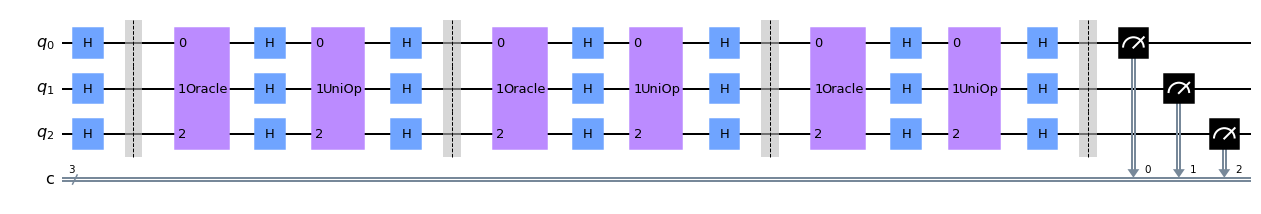
\includegraphics[scale=0.35]{img/Qiskit/StaggeredQW/Search/Circuits/StagSearchCircuit_N3_M0_S3.png}
	\caption{Qiskit circuit for the search problem using the staggered quantum walk model, for a complete graph of size $N=8$, with $3$ steps and a value of $\theta = \frac{\pi}{2}$.}
	\label{fig:stagSearchCircQistkit}
\end{figure}
Similar to previous examples, the circuit begins with the uniform superposition
achieved through Hadamard gates. The next operation of the search problem is
the oracle, which was implemented through the use of Qiskit's \textit{diagonal}
function that produces a circuit similar to the one in figure
\ref{fig:groverOracleCircuitQistkit}.\par

Next, an analogue of Grover's diffusion operator is applied, where the
operation named \textit{UniOp} is a diagonal matrix, easily translated to
Qiskit as is shown in figure \ref{fig:stagSearchUniOpCircQistkit}.  
\begin{figure}[!h]
	\centering
	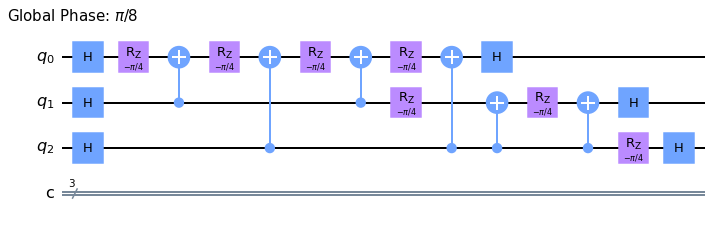
\includegraphics[scale=0.40]{img/Qiskit/StaggeredQW/Search/Circuits/StagUniOpCircuit_N3_M0_S3.png}
	\caption{Qiskit circuit of the  diagonal diffusion operator in the staggered quantum walk search problem, for a complete graph of size $N=8$ and a value of $\theta = \frac{\pi}{2}$.}
	\label{fig:stagSearchUniOpCircQistkit}
\end{figure}
This circuit is very similar to the one in figure
\ref{fig:groverDiffCircuitQistkit}, the difference being that in the staggered
quantum walk search model one can control the value of $\theta$, as can be seen
in equation \ref{eq:unmodEvolOperatorStagSearch}, which influences how fast
maxmimum probability of the marked element is achieved. Since Grover's
algorithm is optimal, a value of $\theta=\frac{\pi}{2}$ yields a diffusion
circuit equal to the one in figure \ref{fig:groverDiffCircuitQistkit}, implying
that the staggered quantum walk is a more general model of quantum searching.\par

Finally, measurement is performed and the resuls for several steps of the walk
are shown in figure \ref{fig:stagSearchResultsToronto}.  
\begin{figure}[!h]
	\centering
	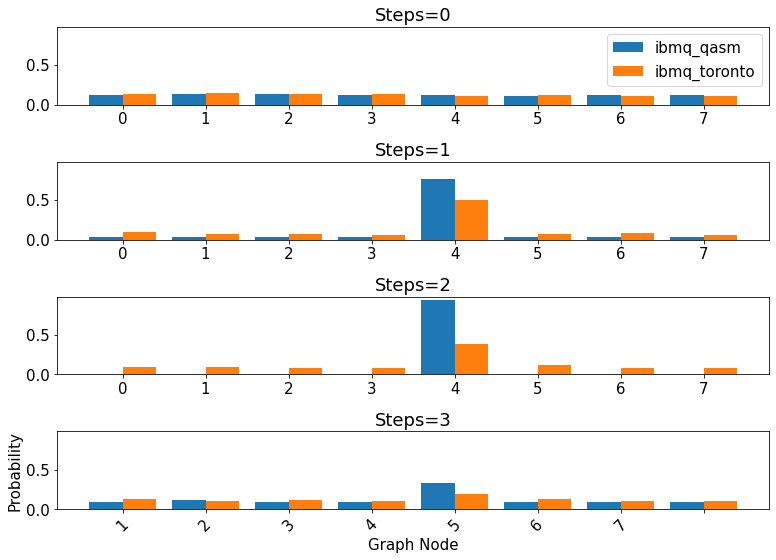
\includegraphics[scale=0.40]{img/Qiskit/StaggeredQW/Search/stagSearchToronto_N3_S0123.png}
	\caption{Probability distributions of the staggered quantum walk search problem for several steps, in a complete graph of size $N=8$. The blue bar plot represents a circuit run in the QASM simulator, and the orange bar plot on IBM's Toronto backend.}
	\label{fig:stagSearchResultsToronto}
\end{figure}
The circuit for each step of the walk was run both in the \textit{QASM}
simulator and IBM's backend named Toronto. The experiment was performed with
$3000$ shots in both cases, and the probability distributions show that this
model is indeed more suited for a NISQ computer than the previous case.
However, unlike the simulator, maximum probability of the marked vertex was
achieved withing $1$ step of the walk instead of the predicted $2$ steps, as
was the case of the Grover algorithm. Looking at the $1$ step case in the
simulator, one can see that the probability of vertex $\ket{4}$ is very close
to the maximum, while the circuit has about half of the operations of the $2$
step case. This means it is not surprising that the smaller circuit produces
higher results for the probability of the marked vertex. 
%TODO: Talvez melhorar as fidelidades com o intervalo de confianca. 
This can be further confirmed by the fidelities of each of the states, which
are aproximately $0.954$ and $0.780$ for $1$ step and $2$ steps, respectively,
implying that the former circuit produces better results because of the number
of operations, even though that the latter should theoretically yield the
highest probability.\par 

Even though these results are a great improvement to the search problem using
the coined quantum walk, the staggered model is still discrete, meaning its
circuit will increase in depth as the number of steps increases. This can be
avoided by turning again to the continuous-time quantum walk, whose circuit
remains constant with time.  However, for the searching problem, the
continuous-time model might not have the best results, because it will need
iterations due to the Suzuki-Trotter approximation and it will also require
extra operations to implement the oracle, which was not the case in the pure
dynamics example of section \ref{sec:ContQiskit}.

\subsection{Continuous}
As was seen in section \ref{sec:ContSearchSimul}, the unitary operator
associated with the continuous time quantum walk model can be modified as to
mark an element for amplitude amplification
\begin{equation}
	U'(t) = e^{iH't} = \phi(t)e^{-i(\gamma A+O)t},
	\label{eq:qiskitU'}
\end{equation}
where $\phi(t)$ is a global phase, $A$ is the adjacency matrix and the oracle
is defined as 
\begin{equation}
	O = \sum_{m \in M} \ket{m}\bra{m},
\end{equation}
where $M$ is the set of marked elements.\par

This section will focus on constructing and analyzing the circuit form of the
continuous-time quantum walk search problem, which will be performed over a
complete graph whose adjacency matrix is
\begin{equation}
  A = 	\begin{pmatrix}
	  0 & 1 &  \cdots & 1 & 1\\
	  1 & 0 & \cdots & 1 & 1\\
	   \vdots & \vdots  & \vdots & \vdots& \vdots\\
	  1 & 1 & \cdots & 0 & 1\\ 
	  1 & 1 & \cdots & 1 & 0\\ 
	\end{pmatrix}.
\end{equation}
which is simply a matrix with all entries set to $1$, except the diagonal.\par

The first step is to borrow the diagonal definition of the adjacency matrix
from equation \ref{eq:qiskitContQWAdj} 
\begin{equation}
    A = F^{\dagger} \Lambda F,
    \label{eq:qiskitContSearchAdj}
\end{equation}
and use the Suzuki-Trotter expansion
\begin{equation}
	e^{i(H_0+H_1)t}=\lim_{r \rightarrow \infty}(e^{i\frac{H_0t}{r}}e^{i\frac{H_1t}{r}})^r ,
\end{equation}
to decompose the operator in equation \ref{eq:qiskitU'} 
\begin{equation}
	e^{i(\gamma A+O)t} =\lim_{r \rightarrow \infty}(F^{\dagger} e^{i\gamma\frac{\Lambda t}{r}} F e^{i\frac{Ot}{r}})^r, 
	\label{eq:suzTrotter}
\end{equation}
which can be easily translated into circuit form as in figure
\ref{fig:contSearchCircuit}. 
\begin{figure}[!h]
	\[ \Qcircuit @C=1.8em @R=1.5em {& & & &  \mbox{Repeat r times} & &\\
	&  {/^{\otimes n}} \qw &\gate{\mbox{H}}  & \gate{\mbox{$e^{i\frac{Ot}{r}}$}} & \gate{\mbox{F}} &\gate{\mbox{$e^{i\gamma\frac{\Lambda t}{r}}$}} & \gate{\mbox{F$^{\dagger}$}} &\qw \gategroup{2}{4}{2}{7}{.8em}{--}
		          } \]
	\centering
 	\caption{General circuit for the search problem using the continuous-time quantum walk model.}
	\label{fig:contSearchCircuit}
\end{figure}\par
Consider the case of a graph of size $N=2^3=8$ and trotter number of $r=1$. The
corresponding Qiskit circuit is as shown in figure \ref{fig:contSearchCircuit}.
\begin{figure}[!h]
	\centering
	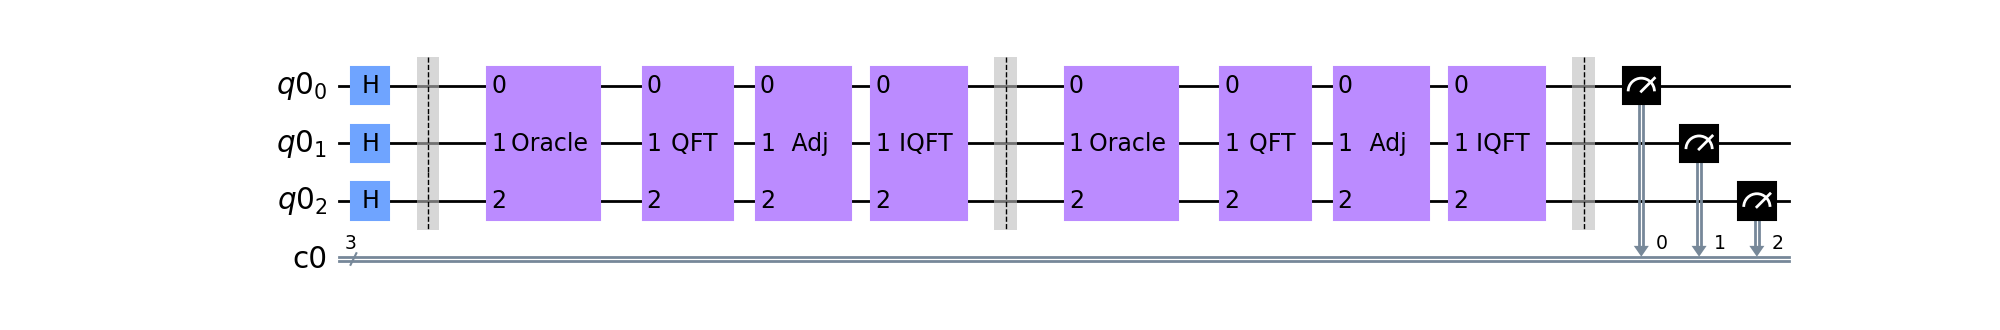
\includegraphics[scale=0.30]{img/Qiskit/ContQuantumWalk/Search/Circuits/circContSearch_N3_S2.png}
	\caption{Qiskit circuit for the search problem using the continuous-time quantum walk model, for a complete graph of size $N=8$, time $t$ and a value of $\gamma = \frac{1}{8}$.}
	\label{fig:contSearchCircQistkit}
\end{figure}
The system starts out in an uniform superposition followed by the application
of the oracle operator as can be seen in figure
\ref{fig:contSearchOracleCircQistkit}. Note that the circuit was obtained by
using Qiskit's \textit{diagonal} function that takes the diagonal entries of
the operator corresponding to the oracle that was defined in equation
\ref{eq:suzTrotter}. 
\begin{figure}[!h]
	\centering
	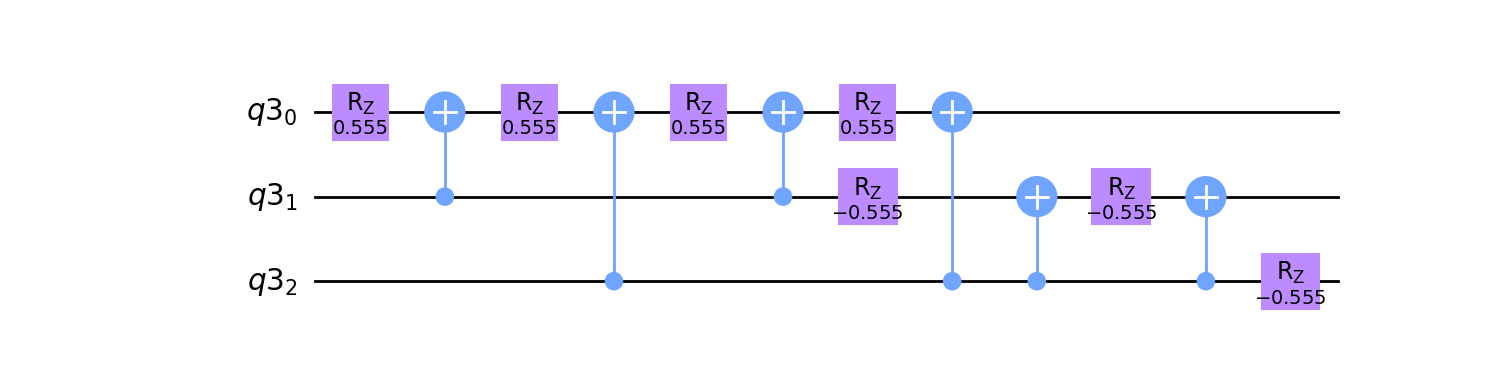
\includegraphics[scale=0.30]{img/Qiskit/ContQuantumWalk/Search/Circuits/circOracle_N3_S2.png}
	\caption{Qiskit circuit of the  diagonal oracle operator in the continuous-time quantum walk search problem, for a complete graph of size $N=8$, marked element $\ket{m}=\ket{4}$ and time $t=\frac{\pi}{2} \sqrt{8}$.}
	\label{fig:contSearchOracleCircQistkit}
\end{figure}\par

The following operation will be the QFT, but because a
complete graph is considered, the AQFT can be used with a degree of $m=2$,
which means the circuit will simply be Hadamard transforms, thus reducing
circuit depth.\par

Lastly, the operator associated with the adjacency matrix is shown in figure
\ref{fig:contSearchAdjCircQistkit}. Since $A$ is the diagonal adjacency matrix
of a complete graph, it is easily implemented using the aforementioned
\textit{diagonal} function.
\begin{figure}[!h]
	\centering
	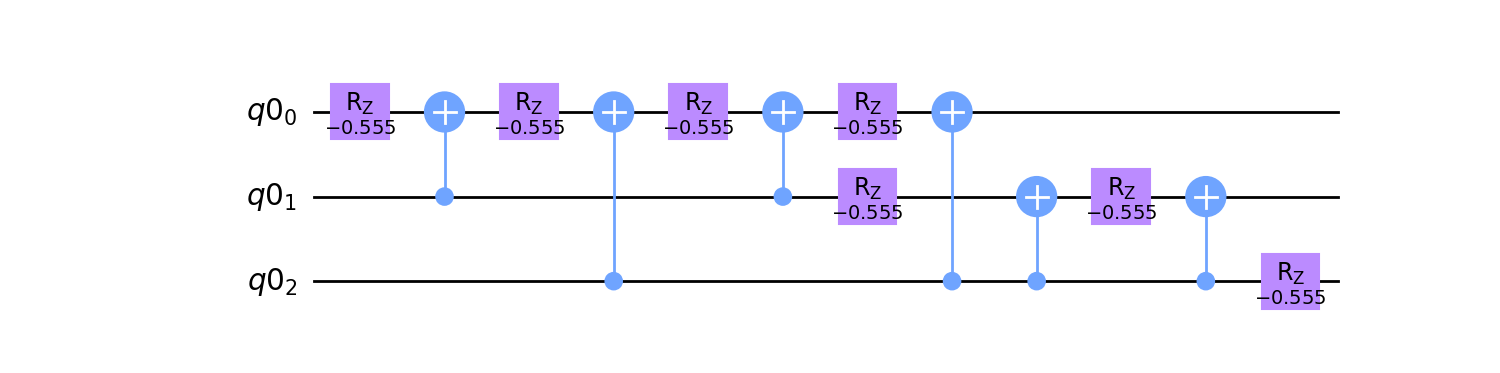
\includegraphics[scale=0.30]{img/Qiskit/ContQuantumWalk/Search/Circuits/circAjd_N3_S2.png}
	\caption{Qiskit circuit of the  diagonal operator associated with the adjacency matrix in the continuous-time quantum walk search problem, for a complete graph of size $N=8$, marked element $\ket{m}=\ket{4}$, time $t=\frac{\pi}{2} \sqrt{8}$ and $\gamma = \frac{1}{8}$.}
	\label{fig:contSearchAdjCircQistkit}
\end{figure}\par

Finally, the results of circuit measurement can be seen in figure
\ref{fig:contSearchResultCircQistkit}.  Even though circuit depth does not
scale up with time, introducing the oracle operation to the continuous-time
quantum walk model appears to make the circuit hard to run in a NISQ computer.
Note that, theoretically, $2$ iterations of the Suzuki-Trotter expansion are
needed for maximum probability of the marked vertex to be achieved in optimal
time. 
\begin{figure}[!h]
	\centering
	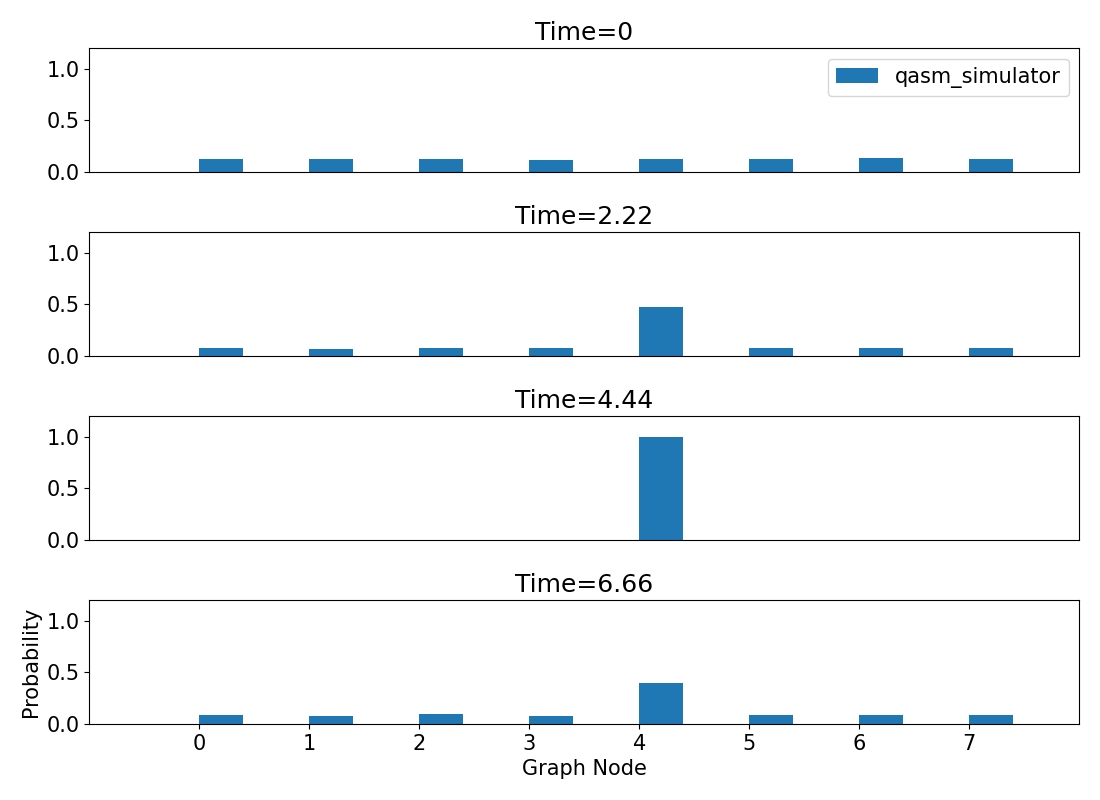
\includegraphics[scale=0.40]{img/Qiskit/ContQuantumWalk/Search/ContQW_N3_S2.png}
	\caption{Probability distributions of the continuous-time quantum walk search problem for several time intervals, in a complete graph of size $N=8$. The blue bar plot represents a circuit run in the QASM simulator, and the orange bar plot on IBM's Toronto backend.}
	\label{fig:contSearchResultCircQistkit}
\end{figure}
In practice, however, greater probability for this element is achieved when
only $1$ iteration is performed since the smaller circuit seems to produce a
greater fidelity of $0.71$, when compared to a fidelity of $0.59$ for the $2$
iteration case. The approximate quantum Fourier transform also has a positive
impact, increasing fidelity from $0.60$ when the full QFT circuit is used, to
the aforementioned $0.71$ when only Hadamard transformations are performed.\par
In conclusion, when comparing the several quantum walk models studied in
previous sections, the coined quantum walk seems to be the least suited for
running the search problem in NISQ computers, followed by the continuous-time
model which has the advantage of not scaling with time, but produces a circuit
slightly too large to achieve fidelities which rival the staggered quantum
walk. The latter appears to perform the best because, even though its discrete
nature requires several iterations, the circuit depth does not appear to
introduce a drastic amount of noise in the $N=8$ case. 

\end{document}
